\section{Evaluation}
\label{sec:evaluation}

We report accuracy as test NRMSE, a normalized error for which lower is better
and where one means predicting the mean. Three ways of turning the shot record
into features are compared throughout. EV averages all shots of a step into one
clean feature vector. Raw keeps every shot as its own noisy example. Grouped is
our method and sits between them. A fourth entry, Cov-EV, is a control that adds
an independently tuned covariance penalty to plain averaging. We summarize the
benefit of Grouped as the paired difference EV minus Grouped, so a positive
value means Grouped is more accurate. Each difference comes with a $95\%$
confidence interval. An interval above zero provides evidence of a positive
mean improvement; an interval containing zero is inconclusive. The balanced
setting spends the fixed budget on $500$ time steps with $20$ shots each.

\subsection{Balanced setting}

At the balanced budget, Grouped lowers mean NRMSE relative to EV on all four
tasks (Table~\ref{tab:balanced}, Fig.~\ref{fig:operating}). The improvement is
$0.0138$ on Mackey--Glass ($95\%$ CI $[-0.0023, 0.0300]$), $0.0848$ on Santa Fe
laser ($[0.0174, 0.1522]$), $0.0349$ on R\"ossler ($[0.0139, 0.0559]$), and
$0.0360$ on sunspots ($[0.0103, 0.0616]$). The interval stays above zero on the
two real-world datasets, Santa Fe laser and sunspots, and on R\"ossler. Only
Mackey--Glass is inconclusive.

\begin{table}[t]
\caption{Mean test NRMSE at the balanced setting. Repeated measurement trials
are averaged within each of five separate trajectories or windows. Lower
values are better.}
\label{tab:balanced}
\centering
\scriptsize
\setlength{\tabcolsep}{1.7pt}
\begin{tabular}{lrrrrrr}
\toprule
Task & Class. & Ideal & EV & Grouped & Raw & Cov-EV \\
\midrule
\QAIBalancedTableRows
\bottomrule
\end{tabular}
\end{table}

Santa Fe laser shows the largest effect. Grouped reduces the error from $0.764$
to $0.680$, and all five disjoint test windows favor Grouped. When $k$ and the
ridge strength are tuned together, the search lands on $k=10$ most often and
on an intermediate scale, neither Raw nor EV, in $94\%$ of repeated trials.
Cov-EV reaches $0.677$, almost the same as Grouped, which already suggests that
the gain is a regularization effect rather than new physical information. The
gain also depends on how the budget is spent. On Santa Fe it shrinks from
$0.143$ with $40$ shots per step to $0.010$ with $10$ shots per step because
grouping has more shots to reorganize when shots are plentiful.

We also compare an ideal noise-free reservoir with a classical baseline that
uses identical preprocessing. The quantum reservoir is worse on Mackey--Glass
and sunspots, better on Santa Fe, and inconclusive on R\"ossler. Our claims are
therefore about organizing a chosen reservoir record, not quantum advantage.
The preferred aggregation scale varies across tasks, trajectories, circuit
settings, measurement draws, and grouping assignments, and EV is occasionally
best. Equation~\eqref{eq:loss-decomposition} explains this variation: changing
$k$ changes which feature combinations the readout is discouraged from using,
not merely the strength of that regularization. Raw is less accurate than
Grouped on all four task means.

\begin{figure}[t]
  \centering
  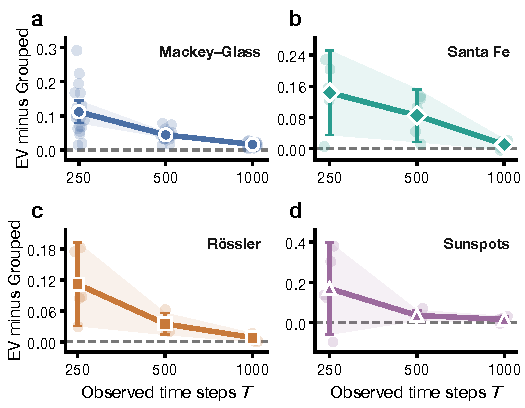
\includegraphics[width=\columnwidth]{fig3_regime_map.pdf}
  \caption{\fontsize{7.25}{8.0}\selectfont When aggregation helps most, at a fixed budget of ten thousand
  circuit executions. Each panel is one task. The vertical axis shows how much
  Grouped improves on full averaging, measured as the EV error minus the
  Grouped error, so a value above the dashed zero line means Grouped wins and a
  value on the line means a tie. Moving right spends the same budget on more
  time steps and therefore fewer shots at each step, from $40$ shots at $250$
  steps to $10$ shots at $1000$ steps. In every task the improvement is largest
  on the left and shrinks toward zero on the right. The message is simple.
  Grouping helps most when each step is measured many times and the series is
  short, because that is exactly when full averaging wastes the most training
  examples. Points are trajectory or window units, and markers with bars are
  means with $95\%$ intervals.}
  \label{fig:regimes}
\end{figure}

\subsection{Trading time steps against shots}

Figure~\ref{fig:regimes} compares three ways of spending the fixed budget. With
$40$ shots at each of $250$ time steps, Grouped improves every task by
$0.086$ to $0.170$. The interval stays above zero for Mackey--Glass, Santa Fe
laser, and R\"ossler, while the sunspot result varies across windows. When the
same budget is spread over $1000$ time steps with only $10$ shots each, the
gains shrink to between $0.008$ and $0.016$, and the interval stays above zero
only for Mackey--Glass and sunspots.

\subsection{Why the gain is regularization}

Cov-EV keeps EV features and adds a penalty based on how the shots fluctuate
together. At the balanced setting its mean error is $0.0021$ to $0.0116$ NRMSE
below Grouped, and only the R\"ossler interval excludes zero. This near-match
supports the regularization mechanism in Eq.~\eqref{eq:loss-decomposition}
rather than extra device information (Fig.~\ref{fig:controls}). Raw is less
accurate than EV on Mackey--Glass and R\"ossler and inconclusive on the two
real-world datasets. At fixed $k$, the exact two-term loss reproduces the
Grouped ridge fit to numerical precision; Cov-EV independently tunes the
strength of the full shot-covariance penalty.

Grouping is also robust to how the groups are drawn. Across twenty repeated
settings the average improvements are $-0.0064$ on Mackey--Glass, $0.1103$ on
Santa Fe laser, $0.0177$ on R\"ossler, and $0.0493$ on sunspots. Only the
sunspot interval stays above zero, reflecting the wide variation across
settings. Fixing one grouping across time instead of reshuffling at every step
changes the error by at most $0.0021$ NRMSE, with every interval containing
zero. The grouping convention therefore matters far less than ordinary
run-to-run variation. Figure~\ref{fig:controls} collects these controls.

\begin{figure}[t]
  \centering
  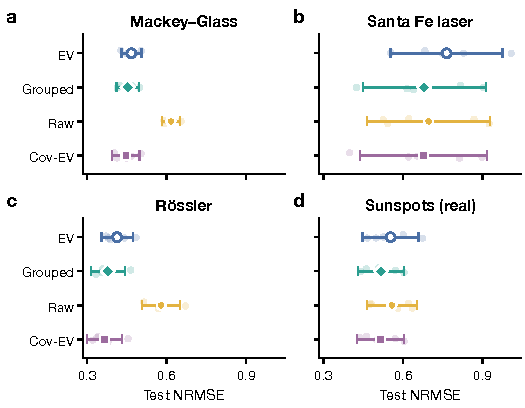
\includegraphics[width=\columnwidth]{fig4_controls_compact.pdf}
  \caption{\fontsize{7.25}{8.0}\selectfont Why the gain is regularization, shown task by task. Each panel places
  the four methods on the same error axis, where lower is better. Grouped (teal
  diamond) and Cov-EV (purple square) sit lowest and almost on top of each other
  on every task, EV (open circle) is behind them, and Raw (yellow, individual
  shots) is worst. The near-match between Grouped and Cov-EV is the key point.
  Cov-EV adds Grouped's fluctuation penalty directly to full averaging, so when
  it reaches the same error the benefit of grouping is regularization of the
  readout rather than extra information from the device. Faint points are the
  five trajectory or window means after repeated measurement trials are
  averaged within each unit. Markers and bars show the means and their $95\%$
  intervals. The order from top to bottom is EV, Grouped, Raw, and Cov-EV.}
  \label{fig:controls}
\end{figure}

\subsection{Transfer to hardware}

Figure~\ref{fig:hardware} reports the unmitigated hardware results. Grouped
improves every task, with mean gains from $0.038$ to $0.153$ NRMSE on
\emph{ibm\_fez} and from $0.031$ to $0.103$ on \emph{ibm\_marrakesh}. On Santa
Fe laser, the error falls from $0.750$ to $0.711$ on \emph{ibm\_fez} and from
$0.744$ to $0.713$ on \emph{ibm\_marrakesh}. Grouped is more accurate in $19$
of $20$ measurement blocks on each processor.

\begin{figure}[!b]
  \centering
  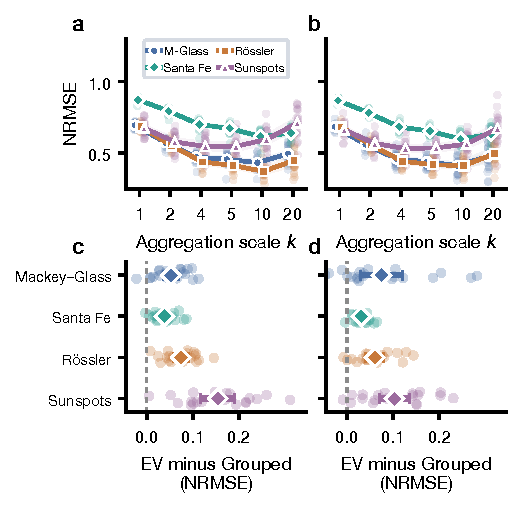
\includegraphics[width=\columnwidth]{fig5_hardware.pdf}
  \caption{\fontsize{7.25}{8.0}\selectfont The same effect on real hardware, on two processors. A separate
  ten-qubit reservoir was run without error mitigation on \emph{ibm\_fez} and
  \emph{ibm\_marrakesh}. For each task and processor, one acquisition of $400$
  shots at each of $T=500$ time steps was split into twenty disjoint records
  with $N=20$. (a,b)~The aggregation spectrum. On both devices the development
  error traces the same U shape over the aggregation scale $k$, so an
  intermediate scale again beats both endpoints on every task. (c,d)~The
  improvement per task, measured as the EV error minus the Grouped error, where
  the dashed line is a tie and points to its right favor Grouped. Grouped is
  more accurate on all four tasks on both machines. Faint points are the
  individual measurement blocks, and each colored marker with a bar is the mean
  with its $95\%$ interval. These intervals describe variation among the blocks
  of a single acquisition, not across independent hardware campaigns.}
  \label{fig:hardware}
\end{figure}
